

\section{USB}

通用串行总线(英语:Universal Serial Bus,缩写USB)是连接计算机系统与外部设备的一种串口总线标准,也是一种输入输出接口的技术规范,被广泛地应用于个人电脑和移动设备等信息通讯产品,并扩展至摄影器材、数字电视(机顶盒)、游戏机等其它相关领域。

多媒体电脑刚问世时,外接式设备的传输界面各不相同,如打印机只能接LPT port、调制解调器只能接RS232、鼠标键盘只能接PS/2等。繁杂的界面系统,加上必须安装驱动程序并重启才能使用的限制,都不免造成用户的困扰。因此,创造出一个统一且支持热插拔的外接式传输界面,便成为无可避免的趋势。
USB最初是由英特尔与微软倡导发起,其最大的特点是支持热插拔和即插即用。当设备插入时,主机枚举到此设备并加载所需的驱动程序,因此在使用上远比PCI和ISA总线方便。
USB在速度上远比并行端口(例如EPP、LPT)与串行接口(例如RS-232)等传统电脑用标准总线快上许多。USB 1.1的最大传输带宽为12Mbps,USB 2.0的最大传输带宽为480Mbps。USB 3.0为5Gbps。

USB的设计为非对称式的,它由一个主机控制器和若干通过集线器设备以树形连接的设备组成。一个控制器下最多可以有5级Hub,包括Hub在内,最多可以连接128个设备,因为在设计时是使用7位寻址字段,二的七次方就等于128,一般人说USB连接127个是指连接(某一设备)时需扣除一个连接主机的USB接头,而一台计算机可以同时有多个控制器。和SPI-SCSI等标准不同,USB集线器不需要终结器。

USB的连接器分为A、B两种,分别用于主机和设备;其各自的小型化的连接器是Mini-A和Mini-B,另外还有Mini-AB(可同时支持Mini-A及Mini-B)的插口。
\begin{figure}[ht]
	\begin{center}
		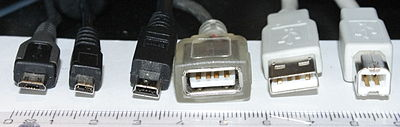
\includegraphics[keepaspectratio,width=0.5\paperwidth]{Hardwares/usb-connectors.jpg}
	\caption{USB连接器类型}
	从左到右分别为:micro-b plug, 非USB(UC-E6,私有),mini-B plug, A receptacle, A plug, B plug。
	\label{fig:USBconnectors}
	\end{center}
\end{figure}

\begin{figure}[ht]
	\begin{center}
		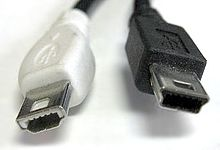
\includegraphics[keepaspectratio,width=0.5\paperwidth]{Hardwares/Mini_usb_AB.jpg}
	\caption{USB mini连接器类型}
	从左到右分别为:mini-A plug,mini-B plug。
	\label{fig:USBconnectors}
	\end{center}
\end{figure}

USB可以连接的外设有鼠标、键盘、游戏手柄、游戏杆、扫描仪、数码相机、打印机、硬盘和网络部件。对数码相机这样的多媒体外设USB已经是缺省接口;由于大大简化了与计算机的连接,USB也逐步取代并行接口成为打印机的主流连接方式。2004年已经有超过1亿台USB设备;到2007年时,高清晰度数字视频外设是仅有的USB未能染指的外设类别,因为他需要更高的传输速率。


USB实装论坛(USB Implementers Forum,USB-IF)负责USB标准制订,其成员包括:苹果电脑、惠普、NEC、微软和英特尔。

2001年底,USB-IF公布了USB 2.0规范,增加更高的数据传输速率480 Mbit/s(现在称作Hi-Speed)。与之前的USB 0.9、USB 1.0和USB 1.1一样,该规范完全向后兼容。随后,USB-IF公布了USB On-The-Go(USB OTG,当前版本:1.0a)作为USB 2.0规范的补充标准,使其能够用于在便携设备之间直接交换数据。

\begin{figure}[ht]
	\begin{center}
		
\includegraphics[keepaspectratio,width=0.5\paperwidth]{Hardwares/usb-logo.png}
	\caption{USB三叉戟Logo}
	代表对USB 2.0性能的支持
	\label{fig:usb-trident-logo}
	\end{center}
\end{figure}

\begin{figure}[ht]
	\begin{center}
		
\includegraphics[keepaspectratio,width=0.5\paperwidth]{Hardwares/usb-hi-speed-logo.png}
	\caption{Hi-speed(USB 2.0) Logo}
	\label{fig:usb-high-speed-logo}
	\end{center}
\end{figure}

\begin{figure}[ht]
	\begin{center}
		
\includegraphics[keepaspectratio,width=0.5\paperwidth]{Hardwares/usb-super-speed-logo.png}
	\caption{Super-speed(USB 3.0) Logo}
	\label{fig:usb-super-speed-logo}
	\end{center}
\end{figure}


2007年1月4日,USB-IF颁布了Micro-USB的插头标准。该标准将在许多新型智能手机和PDA上替代Mini-USB。Micro-USB插头的插拔寿命为10,000次,比Mini-USB插头高度减半,宽度相差无几。OMTP组织最近宣布,Micro-USB将成为移动设备数据和电源的标准接口。

USB 3.0于2008年11月释出。USB 3.0支持全双工,比USB 2.0多了数个触点,并采用发送列表区段来进行数据发包。USB 3.0暂定的供电标准为900mA,且支持光纤传输,设计“Super Speed”传输速度为5Gbit/s,若采用光纤则可达到25Gbit/s。USB 3.0的设计兼容USB 2.0与USB 1.1版本,并采用了三级多层电源管理技术,可以为不同设备提供不同的电源管理方案。

现USB标准中,统一为USB 3.0,理论可以向下兼容。一般产商同时提供USB 3(以蓝色特别标示)与USB 2接口,不提供向下兼容USB 2的USB 3接口。


